\chapter{PRESENTACI�N Y AN�LISIS DE RESULTADOS}
\section{Selecci\'on del movimiento de cada equipo deportivo} \label{res:idMov}
\begin{figure}[H]
	\caption{Formulario de movimiento de tenis de mesa}
	\label{fig:frmMovTen}
	\centering
	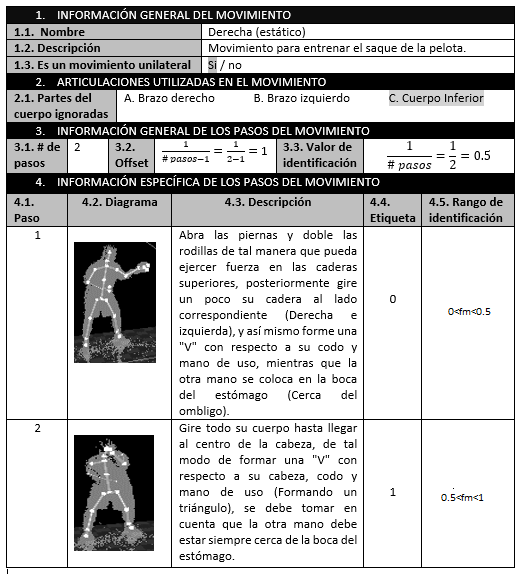
\includegraphics[width=430px,height=360px]{graphics/resultados/movimientoTenis.PNG} \\
	\textbf{Fuente:} Elaborado por el autor de tesis en base a las observaciones del trabajo de campo
\end{figure}
\begin{figure}[H]
	\caption{Formulario de movimiento de animaci\'on}
	\label{fig:frmMovCheer}
	\centering
	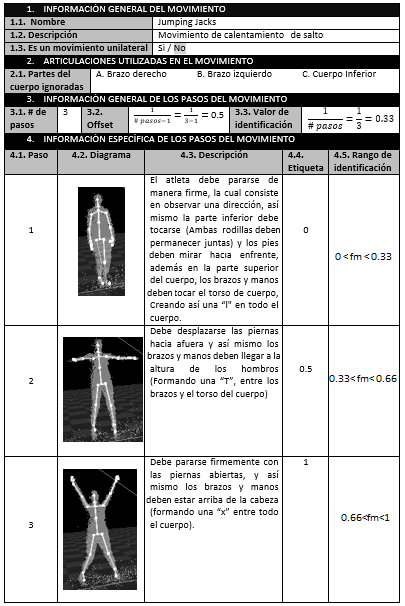
\includegraphics[width=445px,height=600px]{graphics/resultados/movimientoCheerleader.PNG} \\
	\textbf{Fuente:} Elaborado por el autor de tesis en base a las observaciones del trabajo de campo
\end{figure}
\begin{figure}[H]
	\caption{Formulario de movimiento taekwondo}
	\label{fig:frmWhiteMov}
	\centering
	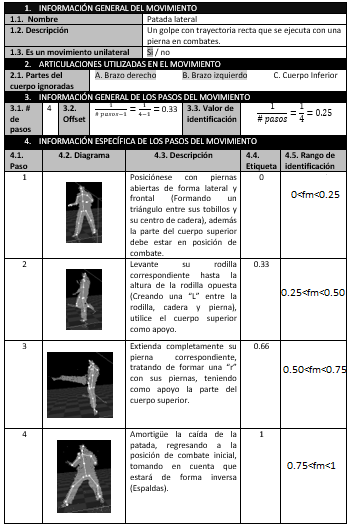
\includegraphics[width=445px,height=600px]{graphics/resultados/movimientoTaekwondo.PNG} \\
	\textbf{Fuente:} Elaborado por el autor de tesis en base a las observaciones del trabajo de campo
\end{figure}
\section{Creaci\'on de rutina del movimiento de cada equipo deportivo} \label{res:idMov}
\begin{figure}[H]
	\caption{Formulario de rutina de animaci\'on}
	\label{fig:frmRoutCher}
	\centering
	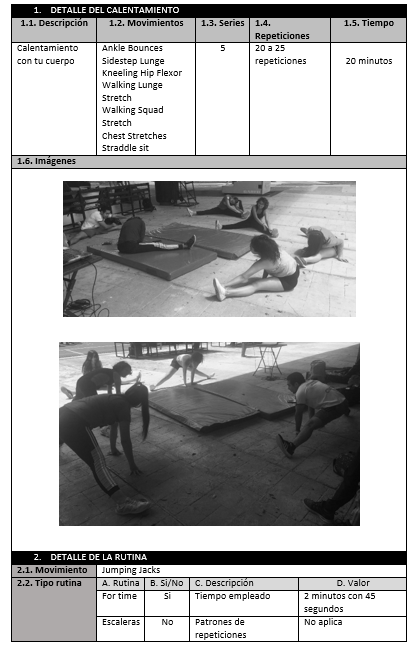
\includegraphics[width=445px,height=550px]{graphics/resultados/rutina-cheerleaders.PNG} \\
	\textbf{Fuente:} Elaborado por el autor de tesis en base a las observaciones del trabajo de campo
\end{figure}
\begin{figure}[H]
	\caption{Formulario de rutina de tenis de mesa}
	\label{fig:frmRoutTen}
	\centering
	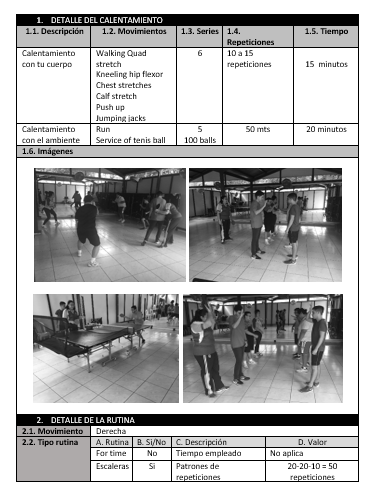
\includegraphics[width=445px,height=600px]{graphics/resultados/rutina-tennis.PNG} \\
	\textbf{Fuente:} Elaborado por el autor de tesis en base a las observaciones del trabajo de campo
\end{figure}
\begin{figure}[H]
	\caption{Formulario de rutina de taekwondo}
	\label{fig:frmRoutTaek}
	\centering
	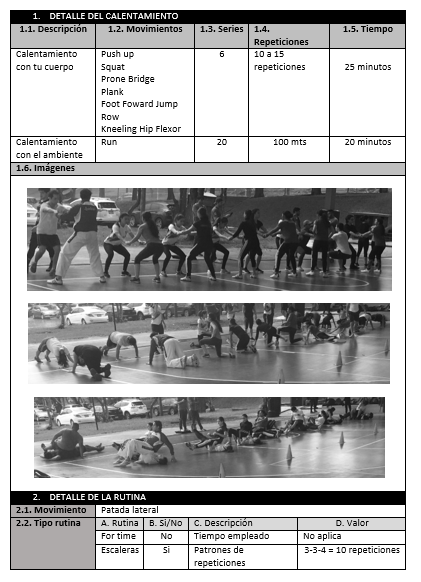
\includegraphics[width=445px,height=600px]{graphics/resultados/rutina-taekwondo.PNG} \\
	\textbf{Fuente:} Elaborado por el autor de tesis en base a las observaciones del trabajo de campo
\end{figure}
\section{Distancias de profundidad recomendadas entre el atleta y el sensor} \label{res:idMov}
\begin{table}[H]
\begin{center}
\caption{Distancias de profundidad con respecto a la cadera central del atleta, tomada a una altura del Kinect de 0.70 mts (Medida a partir del suelo)}
\label{tab:depthCalculation}
\begin{tabular}{lllll}
\hline
\multicolumn{3}{|c|}{Caracter\'isticas generales} & \multicolumn{2}{l|}{\begin{tabular}[c]{@{}l@{}}Distancia de profundidad\\ recomendada entre el \\ usuario y el sensor\end{tabular}} \\ \hline
\multicolumn{1}{|l|}{Deporte} & \multicolumn{1}{l|}{\begin{tabular}[c]{@{}l@{}}Altura promedio\\ (Metros)\end{tabular}} & \multicolumn{1}{l|}{\begin{tabular}[c]{@{}l@{}}Desviaci\'on est\'andar\\ de la altura (metros)\end{tabular}} & \multicolumn{1}{l|}{\begin{tabular}[c]{@{}l@{}}M\'inima\\ (Metros)\end{tabular}} & \multicolumn{1}{l|}{\begin{tabular}[c]{@{}l@{}}M\'axima\\ (Metros)\end{tabular}} \\ \hline
\multicolumn{1}{|l|}{Tenis de mesa} & \multicolumn{1}{l|}{1.302435} & \multicolumn{1}{l|}{0.088683} & \multicolumn{1}{l|}{3.505103} & \multicolumn{1}{l|}{3.990376} \\ \hline
\multicolumn{1}{|l|}{Animaci\'on} & \multicolumn{1}{l|}{1.342471} & \multicolumn{1}{l|}{0.059301} & \multicolumn{1}{l|}{2.763813} & \multicolumn{1}{l|}{3.411942} \\ \hline
\multicolumn{1}{|l|}{Taekwondo} & \multicolumn{1}{l|}{1.373372} & \multicolumn{1}{l|}{0.098490} & \multicolumn{1}{l|}{2.556640} & \multicolumn{1}{l|}{3.869427} \\ \hline
\multicolumn{5}{l}{\textbf{Fuente:} Instrumento \ref{ins:UI:wpf}.\ref{ins:UI:wpf:depth} utilizado en los atletas de construcci\'on y pruebas (ver secci\'on \ref{sj:1t})}
\end{tabular}
\end{center}
\end{table}
